\paragraph[QuizziPedia::Front-End::QML\\::QuestionCheck::Custom]{QuizziPedia::Front-End::QML::QuestionCheck::Custom}
\begin{figure} [ht]
	\centering
	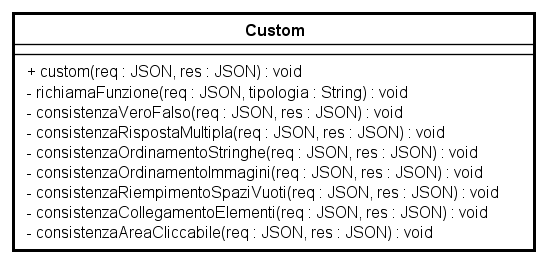
\includegraphics[scale=0.80]{UML/Classi/Front-End/QuizziPedia_Front-End_QML_QuestionCheck_Custom.png}
	\caption{QuizziPedia::Front-End::QML::QuestionCheck::Custom}
\end{figure} \FloatBarrier
\begin{itemize}
	\item \textbf{Descrizione}: questa classe  permette di controllare la validità semantica del codice \textit{QML\ped{G}} relativo alla tipologia di domanda "Custom";
	\item \textbf{Utilizzo}: fornisce le funzionalità per inserire una nuova domanda ad custom nel database e per modificarne una esistente;
	\item \textbf{Relazioni con altre classi}:
	\begin{itemize}
		\item \textbf{IN} \texttt{CheckQML}: classe che fornisce le funzionalità per controllare la validità semantica del codice \textit{QML\ped{G}}.
	\end{itemize}
	\item \textbf{Metodi}:
	\item \textbf{Metodi}:
	\begin{itemize}
		\item \texttt{+} \texttt{custom(req : JSON, res : JSON)} \\
		Questo metodo permette di controllare la semantica del codice \textit{QML\ped{G}}, restituisce un JSON con la domanda valida oppure un JSON contenente un messaggio d'errore. \\
		\textbf{Parametri}:
		\begin{itemize}
			\item \texttt{req : JSON} \\
			Parametro contenente il codice QML scritto dall'utente nell'editor di testo e sintatticamente valido;
			\item \texttt{res : JSON} \\
			Parametro che contiene il JSON specifico per la domanda da creare o un JSON con un messaggio d'errore.
		\end{itemize}
		\item \texttt{-} \texttt{richiamaFunzione(req : JSON, res : JSON, tipologia : String)} \\
		Questo metodo privato permette di richiamare il metodo appropriato per controllare la consistenza delle domande interne alla domanda Custom. \\
		\textbf{Parametri}:
		\begin{itemize}
			\item \texttt{req : JSON} \\
			Parametro contenente il codice QML scritto dall'utente nell'editor di testo e sintatticamente valido;
			\item \texttt{res : JSON} \\
			Parametro che contiene il JSON specifico per la domanda da creare o un JSON con un messaggio d'errore;
			\item \texttt{tipologia: Stirng} \\
			Parametro che indica la tipologia di domanda interna per la scelta corretta del metodo da invocare.
		\end{itemize}
		\item \texttt{-} \texttt{consistenzaVeroFalso(req : JSON, res : JSON)} \\
		Questo metodo privato permette di verificare la consistenza della specifica domanda interna che compone la domanda Custom \\
		\textbf{Parametri}:
		\begin{itemize}
			\item \texttt{req : JSON} \\
			Parametro contenente il codice QML inerente alla composizione della domanda interna specifica e sintatticamente valida;
			\item \texttt{res : JSON} \\
			Parametro che contiene il JSON specifico per la domanda interna da creare o un JSON con un messaggio d'errore;
		\end{itemize}
		\item \texttt{-} \texttt{consistenzaRispostaMultipla(req : JSON, res : JSON)} \\
		Questo metodo privato permette di verificare la consistenza della specifica domanda interna che compone la domanda Custom \\
		\textbf{Parametri}:
		\begin{itemize}
			\item \texttt{req : JSON} \\
			Parametro contenente il codice QML inerente alla composizione della domanda interna specifica e sintatticamente valida;
			\item \texttt{res : JSON} \\
			Parametro che contiene il JSON specifico per la domanda interna da creare o un JSON con un messaggio d'errore;
		\end{itemize}
		\item \texttt{-} \texttt{consistenzaOrdinamentoStringhe(req : JSON, res : JSON)} \\
		Questo metodo privato permette di verificare la consistenza della specifica domanda interna che compone la domanda Custom \\
		\textbf{Parametri}:
		\begin{itemize}
			\item \texttt{req : JSON} \\
			Parametro contenente il codice QML inerente alla composizione della domanda interna specifica e sintatticamente valida;
			\item \texttt{res : JSON} \\
			Parametro che contiene il JSON specifico per la domanda interna da creare o un JSON con un messaggio d'errore;
		\end{itemize}
		\item \texttt{-} \texttt{consistenzaOrdinamentoImmagini(req : JSON, res : JSON)} \\
		Questo metodo privato permette di verificare la consistenza della specifica domanda interna che compone la domanda Custom \\
		\textbf{Parametri}:
		\begin{itemize}
			\item \texttt{req : JSON} \\
			Parametro contenente il codice QML inerente alla composizione della domanda interna specifica e sintatticamente valida;
			\item \texttt{res : JSON} \\
			Parametro che contiene il JSON specifico per la domanda interna da creare o un JSON con un messaggio d'errore;
		\end{itemize}
		\item \texttt{-} \texttt{consistenzaRiempimentoSpaziVuoti(req : JSON, res : JSON)} \\
		Questo metodo privato permette di verificare la consistenza della specifica domanda interna che compone la domanda Custom \\
		\textbf{Parametri}:
		\begin{itemize}
			\item \texttt{req : JSON} \\
			Parametro contenente il codice QML inerente alla composizione della domanda interna specifica e sintatticamente valida;
			\item \texttt{res : JSON} \\
			Parametro che contiene il JSON specifico per la domanda interna da creare o un JSON con un messaggio d'errore;
		\end{itemize}
		\item \texttt{-} \texttt{consistenzaCollegamentoElementi(req : JSON, res : JSON)} \\
		Questo metodo privato permette di verificare la consistenza della specifica domanda interna che compone la domanda Custom \\
		\textbf{Parametri}:
		\begin{itemize}
			\item \texttt{req : JSON} \\
			Parametro contenente il codice QML inerente alla composizione della domanda interna specifica e sintatticamente valida;
			\item \texttt{res : JSON} \\
			Parametro che contiene il JSON specifico per la domanda interna da creare o un JSON con un messaggio d'errore;
		\end{itemize}
		\item \texttt{-} \texttt{consistenzaAreacliccabile(req : JSON, res : JSON)} \\
		Questo metodo privato permette di verificare la consistenza della specifica domanda interna che compone la domanda Custom \\
		\textbf{Parametri}:
		\begin{itemize}
			\item \texttt{req : JSON} \\
			Parametro contenente il codice QML inerente alla composizione della domanda interna specifica e sintatticamente valida;
			\item \texttt{res : JSON} \\
			Parametro che contiene il JSON specifico per la domanda interna da creare o un JSON con un messaggio d'errore;
		\end{itemize}
	\end{itemize}
\end{itemize}

